\documentclass{standalone}
\usepackage{graphicx}
\usepackage{siunitx}
\usepackage{tikz} % To generate the plot from csv
\usepackage{varwidth}
\usepackage[normalem]{ulem}
\usetikzlibrary{shapes,arrows}
\usetikzlibrary{backgrounds}
\usetikzlibrary{matrix, positioning, fit}
\usetikzlibrary{patterns}
\definecolor{forestgreen}{rgb}{0.0, 0.5, 0.0}
\usetikzlibrary{decorations.pathreplacing}
\tikzstyle{smallcircle} =[fill=black!100, text=white, circle, inner sep=1pt, minimum size=0.1em]
\tikzstyle{ourcircle} = [draw, semicircle, inner sep=0pt,minimum size=2pt]
\tikzstyle{dullblock} = [draw, fill=black!20, circle, minimum height=2em, minimum width=2em]
\tikzstyle{block} = [draw=black, rounded corners, thick, line width=0.3mm, rectangle, minimum height=10em, minimum width=7em]
\tikzstyle{blocksmall} = [draw=black, thick, line width=0.5mm, rectangle, minimum height=6em, minimum width=3em, fill=white]
\tikzstyle{group} = [draw=black, line width=0.3mm, rectangle, minimum height=2em, minimum width=2em]
\tikzstyle{textblock} = [draw, fill=black!20, rectangle, rounded corners]
\tikzstyle{rectblock} = [draw, rectangle, minimum height=1.3em]
\tikzstyle{plain} = []
\tikzstyle{decisionblock} = [draw, diamond, fill=black!20]
\tikzstyle{input} = [draw, thick, fill=blue!20, circle, minimum size=1pt]
\tikzstyle{output} = [draw, fill=blue!20, circle, minimum size=1pt]
\tikzstyle{pinstyle} = [pin edge={to-,thin,black}]
\tikzset{toprule/.style={%
        execute at end cell={%
            \draw [line cap=rect,#1] (\tikzmatrixname-\the\pgfmatrixcurrentrow-\the\pgfmatrixcurrentcolumn.north west) -- (\tikzmatrixname-\the\pgfmatrixcurrentrow-\the\pgfmatrixcurrentcolumn.north east);%
        }
    },
    bottomrule/.style={%
        execute at end cell={%
            \draw [line cap=rect,#1] (\tikzmatrixname-\the\pgfmatrixcurrentrow-\the\pgfmatrixcurrentcolumn.south west) -- (\tikzmatrixname-\the\pgfmatrixcurrentrow-\the\pgfmatrixcurrentcolumn.south east);%
        }
    }
}

\begin{document}

    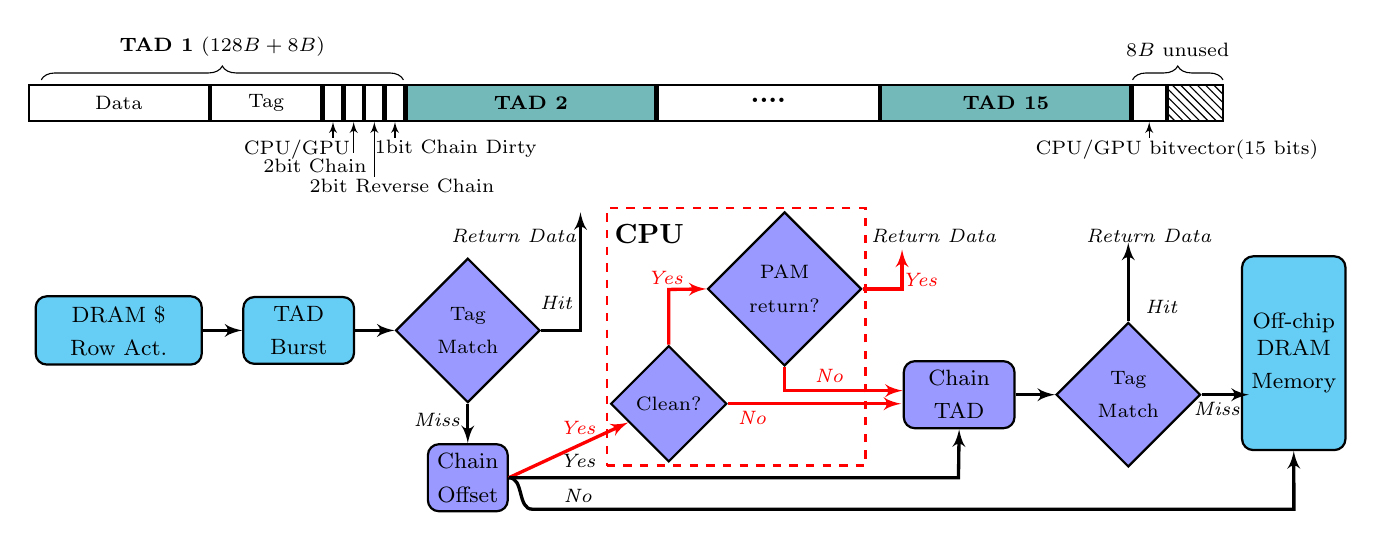
\begin{tikzpicture}[auto, >=latex']
        % We start by placing the blocks
        \node [textblock, thick, minimum width=6em, fill=cyan!60] (act){\begin{varwidth}{4cm} \centering{\footnotesize{DRAM $\$$ \\Row Act.}} \end{varwidth}};
        \node [textblock, thick, right = 0.5cm of act, minimum width=4em, fill=cyan!60] (burst) {\begin{varwidth}{4cm} \centering{\footnotesize{TAD \\Burst}} \end{varwidth}};
        \node [decisionblock, thick, right = 0.5cm of burst, fill=blue!40] (tagmatch) {\begin{varwidth}{4cm} \centering{\scriptsize{Tag\\Match}} \end{varwidth}};
        \node [textblock, thick, below = 0.5cm of tagmatch, fill=blue!40] (chaintable) {\begin{varwidth}{4cm} \centering{\footnotesize{Chain\\Offset}} \end{varwidth}};
        \node [decisionblock, thick, right = 1.8cm of tagmatch.south, fill=blue!40] (clean) {\begin{varwidth}{4cm} \centering{\scriptsize{Clean?}} \end{varwidth}};
        \node [decisionblock, thick, right = 2.1cm of tagmatch, yshift=1.5em, fill=blue!40] (pamreturn) {\begin{varwidth}{4cm} \centering{\scriptsize{PAM \\return?}} \end{varwidth}};
        \node [textblock, thick, right = 1.5cm of pamreturn.south, minimum width=4em, yshift=-1em, fill=blue!40] (chaintad) {\begin{varwidth}{4cm} \centering{\footnotesize{Chain\\TAD}} \end{varwidth}};
        \node [decisionblock, thick, right = 0.5cm of chaintad, , fill=blue!40] (chainmatch) {\begin{varwidth}{4cm} \centering{\scriptsize{Tag\\Match}} \end{varwidth}};
        \node [textblock, thick, right = 0.5cm of chainmatch, minimum height=7em, yshift=1.5em, fill=cyan!60] (mem) {\begin{varwidth}{4cm} \centering{\footnotesize{Off-chip\\DRAM\\Memory}} \end{varwidth}};

        % Arrows
        \draw [->,very thick] (act) -- (burst);
        \draw [->,very thick, red] (chaintable.east) -- (clean);
        \draw [->,very thick] (burst) -- (tagmatch);
        \draw [->,very thick] (tagmatch.south) -- (chaintable.north);
        \draw [->,very thick] (tagmatch.east) to [out=0,in=180] ++(0.5,0) to [out=90,in=-90] ++(0,1.5);
        \draw [->,very thick, red] (clean.north) to [out=90,in=-90] ++(0,0.7) to (pamreturn.west);
        \draw [->,very thick, red] (pamreturn.south)to [out=-90,in=90] ++(0,-0.3) to [out=0,in=180] ++(1.5,0);
        \draw [->,very thick, red] (pamreturn.east) to [out=0,in=180] ++(0.5,0) to [out=90,in=-90] ++(0,0.5);
        \draw [->,very thick, red] (clean.east) to [out=0,in=180] ++(2.2,0);
%        \draw [->,very thick] (chaintable.south) to [out=0,in=180] ++(9.65,0) to (mem.south);
        \draw [->,very thick] (chainmatch.east) to [out=0,in=180] ++(0.6,0);
        \draw [->,very thick] (chaintad.east) -- (chainmatch);
        \draw [->,very thick] (chainmatch.north) to [out=90,in=-90] ++(0,1);
        \draw [->,very thick] (chaintable.east) to [out=0,in=180] ++(5.71,0) to (chaintad.south);
        \draw [->,very thick] (chaintable.east) to [out=0,in=180] ++(0.3,-0.4) to [out=0,in=180] ++(9.67,0) to (mem.south);

        % Groups
        \node [blocksmall,  opacity=0,text opacity=1, draw=white, above = 1cm of clean, minimum height=1em, minimum width=0.2em, xshift=-0.7em, yshift=0.4em] (lblcpu){\textbf{CPU}};
        \node[group, dashed, inner sep = 1pt, line width=0.3mm, draw=red, fit=(clean)(pamreturn)] (cpugroup) {};

        % Labels
        \node [plain, right=0.01em of tagmatch, minimum height=1em, minimum width=1em, yshift=1em, xshift=-0.4em] (lbl1) {\scriptsize{\emph{Hit}}};
        \node [plain, below=0.01em of tagmatch, minimum height=1em, minimum width=1em, xshift=-1.1em] (lbl2) {\scriptsize{\emph{Miss}}};
        \node [plain, below=0.52cm of tagmatch, minimum height=1em, minimum width=1em, xshift=4em] (lbl3) {\scriptsize{\emph{Yes}}};
        \node [plain, below=0.1cm of lbl3, minimum height=1em, minimum width=1em, yshift=0.2em] (lbl4) {\scriptsize{\emph{No}}};
        \node [plain, above=0.01cm of lbl3, minimum height=1em, minimum width=1em, red] (lb15) {\scriptsize{\emph{Yes}}};
        \node [plain, right=0.01em of chainmatch, minimum height=1em, minimum width=1em, yshift=-0.5em, xshift=-0.65em] (lbl5) {\scriptsize{\emph{Miss}}};
        \node [plain, above=3em of lbl5, minimum height=1em, minimum width=1em, yshift=-0.5em, xshift=-2em] (lbl8) {\scriptsize{\emph{Hit}}};
        \node [plain, right=0.01em of clean, minimum height=1em, minimum width=1em, yshift=-0.5em, red] (lbl6) {\scriptsize{\emph{No}}};
        \node [plain, right=2.5em of lbl6, minimum height=1em, minimum width=1em, yshift=1.5em, xshift=-1.5em, red] (lbl7) {\scriptsize{\emph{No}}};
        \node [plain, above=1.8em of clean, minimum height=1em, minimum width=1em, xshift=-0.1em, red] (lbl9) {\scriptsize{\emph{Yes}}};
        \node [plain, above=1.8em of chaintad, minimum height=1em, minimum width=1em, yshift=0.5em, xshift=-1.4em, red] (lbl10) {\scriptsize{\emph{Yes}}};
        \node [plain, above=0.4em of lbl10, minimum height=1em, minimum width=1em, xshift=0.5em] (lbl11) {\scriptsize{\emph{Return Data}}};
        \node [plain, left=9.9em of lbl11, minimum height=1em, minimum width=1em] (lbl12) {\scriptsize{\emph{Return Data}}};
        \node [plain,right =2.5em of lbl11, minimum height=1em, minimum width=1em] (lbl13) {\scriptsize{\emph{Return Data}}};

        % Row Buffer
        \node [rectblock, thick, above = 2.2cm of act, minimum width=6.5em] (data) {\begin{varwidth}{4cm} \centering{\scriptsize{Data}} \end{varwidth}};
        \node [rectblock, thick, right = 0cm of data, minimum width=4em] (tag) {\begin{varwidth}{4cm} \centering{\scriptsize{Tag}} \end{varwidth}};
        \node [rectblock, thick, right = 0cm of tag, minimum width=1pt] (isgpu) {\begin{varwidth}{4cm} \centering{\scriptsize{}} \end{varwidth}};
        \node [rectblock, thick, right = 0cm of isgpu] (chain) {\begin{varwidth}{4cm} \centering{\scriptsize{}} \end{varwidth}};
        \node [rectblock, thick, right = 0cm of chain] (reversechain) {\begin{varwidth}{4cm} \centering{\scriptsize{}} \end{varwidth}};
        \node [rectblock, thick, right = 0cm of reversechain, minimum width=1pt] (chaindirty) {\begin{varwidth}{4cm} \centering{\scriptsize{}} \end{varwidth}};
        \node [rectblock, thick, right = 0cm of chaindirty, minimum width=9em,fill=teal!55] (tad2) {\begin{varwidth}{4cm} \centering{\scriptsize{\textbf{TAD 2}}} \end{varwidth}};
        \node [rectblock, thick, right = 0cm of tad2, minimum width=8em] (row) {\begin{varwidth}{4cm} \centering{\textbf{....}} \end{varwidth}};
        \node [rectblock, thick, right = 0cm of row, minimum width=9em, fill=teal!55] (tad15) {\begin{varwidth}{4cm} \centering{\scriptsize{\textbf{TAD 15}}} \end{varwidth}};
        \node [rectblock, thick, right = 0cm of tad15, minimum width=1.2em] (cg) {\begin{varwidth}{4cm} \centering{} \end{varwidth}};
        \node [rectblock, thick, right = 0cm of cg, minimum width=2em, pattern=north west lines] (dc) {\begin{varwidth}{4cm} \centering{} \end{varwidth}};
        \draw [decorate,decoration={brace,amplitude=5pt},yshift=8.2em, xshift=-2.8em] (0,0.3) -- (4.6,0.3) node [black,midway,yshift=0.5em] {\scriptsize \textbf{TAD 1} ($128B + 8B$)};
        \draw [decorate,decoration={brace,amplitude=5pt},yshift=8.2em, xshift=3.2em] (11.75,0.3) -- (12.9,0.3) node [black,midway,yshift=0.5em] {\scriptsize $8B$ unused};

        \node [plain, below=0.35cm of chain, minimum height=1em, minimum width=1em, xshift=-1.4em] (lbl31){\begin{varwidth}{4cm} \centering{\scriptsize{2bit Chain}} \end{varwidth}};
        \node [plain, below=0.6cm of reversechain, minimum height=1em, minimum width=1em, xshift=1em] (lbl32) {\begin{varwidth}{4cm} \centering{\scriptsize{2bit Reverse Chain}} \end{varwidth}};
        \node [plain, below=0.1cm of chaindirty, minimum height=1em, minimum width=1em, xshift=2.2em] (lbl33) {\begin{varwidth}{4cm} \centering{\scriptsize{1bit Chain Dirty}} \end{varwidth}};
        \node [plain, below=0.1cm of cg, minimum height=1em, minimum width=1em, xshift=1em] (lbl34) {\begin{varwidth}{4cm} \centering{\scriptsize{CPU/GPU bitvector(15 bits)}} \end{varwidth}};
        \node [plain, below=0.1cm of isgpu, minimum height=1em, minimum width=1em, xshift=-1.3em] (lbl35) {\begin{varwidth}{4cm} \centering{\scriptsize{CPU/GPU}} \end{varwidth}};

        \draw [<-] (chain.south) to [out=-90,in=90] ++(0,-0.4);
        \draw [<-] (reversechain.south) to [out=-90,in=90] ++(0,-0.7);
        \draw [<-] (chaindirty.south) to [out=-90,in=90] ++(0,-0.2);
        \draw [<-] (cg.south) to [out=-90,in=90] ++(0,-0.2);
        \draw [<-] (isgpu.south) to [out=-90,in=90] ++(0,-0.2);

    \end{tikzpicture}
\end{document}
